\documentclass[pdflatex,compress]{beamer}

%\usetheme[dark,framenumber,totalframenumber]{ElektroITK}
\usetheme[darktitle,framenumber,totalframenumber]{ElektroITK}

\usepackage{graphicx}

\title{PEMODELAN JARINGAN KOMUNIKASI}
\subtitle{Pengantar Pemodelan Jaringan Komunikasi}

\author{Mifta Nur Farid, S.T., M.T.}

\begin{document}

\maketitle

% ----------------------------------------------------------------------------

\section{Kontrak Perkuliahan}
\subsection{Capaian Pembelajaran Mata Kuliah}
\begin{frame}
	\frametitle{Capaian Pembelajaran Mata Kuliah}
	Mahasiswa mampu menganalisis model dan simulasi dari jaringan komunikasi.
\end{frame}

\subsection{Bahan Kajian}
\begin{frame}
	\frametitle{Bahan Kajian}
	\begin{enumerate}
		\item Dasar Pemodelan dan Simulasi Jaringan
		\item M2M, D2D, model jaringan dan standar jaringan Adhoc IEEE 802.15.4 dan IEEE 802.11
		\item Desain jaringan dan Parameter Protokol
		\item Pemodelan Jaringan menggunakan model matematis
		\item Desain Jaringan dan Parameter Protokol Menggunakan Tool Software Network Simulator
	\end{enumerate}
\end{frame}

\subsection{Pustaka}
\begin{frame}
	\frametitle{Pustaka}
	\begin{enumerate}
		\item Issariyakul, T. \& Hossain, E. (2012). Introduction to Network Simulator NS2. New York: Springer.
		\item Law, A.M. \& Kelton, W. D. (2001). Simulation Modeling and Analysis. New York: McGraw-Hill.
		\item Altman, E. \& Jiménez, T. (2012). NS Network Simulator for Beginners. Berkeley: Morgan \& Claypool
		Publishers.
	\end{enumerate}
\end{frame}

\subsection{Jenis dan Bobot Evaluasi}
\begin{frame}
	\frametitle{Jenis dan Bobot Evaluasi}
	\begin{enumerate}
		\item Kehadiran: 10\%
		\item Tugas: 10\%
		\item Kuis: 15\%
		\item UTS: 20\%
		\item UAS: 20\%
		\item Tugas Besar: 25\%
	\end{enumerate}
\end{frame}
% ----------------------------------------------------------------------------

\section{Pengantar Pemodelan Jaringan Komunikasi}
\subsection{Pendahuluan}
\begin{frame}
	\frametitle{Pendahuluan}
	\begin{itemize}
		\item Manusia berkomunikasi dan saling bertukar informasi sepanjang waktu.
		\item Dalam beberapa dekade terakhir, banyak teknologi yang tercipta untuk membantu proses pertukaran informasi dengan cara yang kreatif dan efisien.
		\item Di antaranya adalah telepon, tv dan radio broadcasting, komputer dan internet, serta teknologi wireless.
		\item Awalnya, teknologi-teknologi tersebut ada dan beroperasi secara mandiri, melakukan tujuannya masing-masing.
	\end{itemize}
\end{frame}

\begin{frame}
	\frametitle{Pendahuluan}
	\begin{itemize}
		\item Kemudian baru-baru ini, teknologi-teknologi tersebut mulai manyatu, dan tidak bisa dipungkiri lagi bahwa hasilnya adalah jaringan telekomunikasi yang kita gunakan saat ini.
		\item Pada mata kuliah ini, jaringan komunikasi akan dijelaskan kembali. Begitu juga dengan model dan layer jaringannya.
		\item Kemudian cara untuk mendisain dan memodelkan sistem jaringan telekomunikasi yang kompleks akan diajarkan. Dilanjutkan dengan melakukan simulasi dari sistem tersebut menggunakan network simulator.
	\end{itemize}
\end{frame}

\subsection{Jaringan Komputer}
\begin{frame}
	\frametitle{Jaringan Komputer}
	\begin{itemize}
		\item Jaringan komputer/ computer network: sekumpulan interkoneksi antar komputer yang bertujuan untuk mengumpulkan, memproses, dan mendistribusikan informasi.
		\item Komputer: workstation, server, router, modems, base station, dan wireless extension point.
		\item Komputer-komputer terhubung dengan communication link: copper cable, fiber optic cable, dan microwave/satellite/radio link.
		\item Jaringan komputer $\rightarrow$ nested dan/atau interkoneksi dari beberapa jaringan $\rightarrow$ internet
		\item Internet: jaringan di dalam jaringan $\rightarrow$ puluhan ribu jaringan yang menginterkoneksikan/ menghubungkan jutaan komputer di seluruh dunia.
	\end{itemize}
\end{frame}

\subsection{Konsep Layering}
\begin{frame}
	\frametitle{Konsep Layering}
	\begin{itemize}
		\item Computer network: sistem yang kompleks.
		\item Untuk memfasilitasi desain dan implementasi yang fleksibel dari sistem tsb $\rightarrow$ konsep layering.
		\item Menggunakan struktur yang berlayer/berlapis, fungsionalitas dari computer network dapat diatur sebagai tumpukan layer.
	\end{itemize}
\end{frame}

\begin{frame}
	\frametitle{Konsep Layering}	
	\begin{center}
		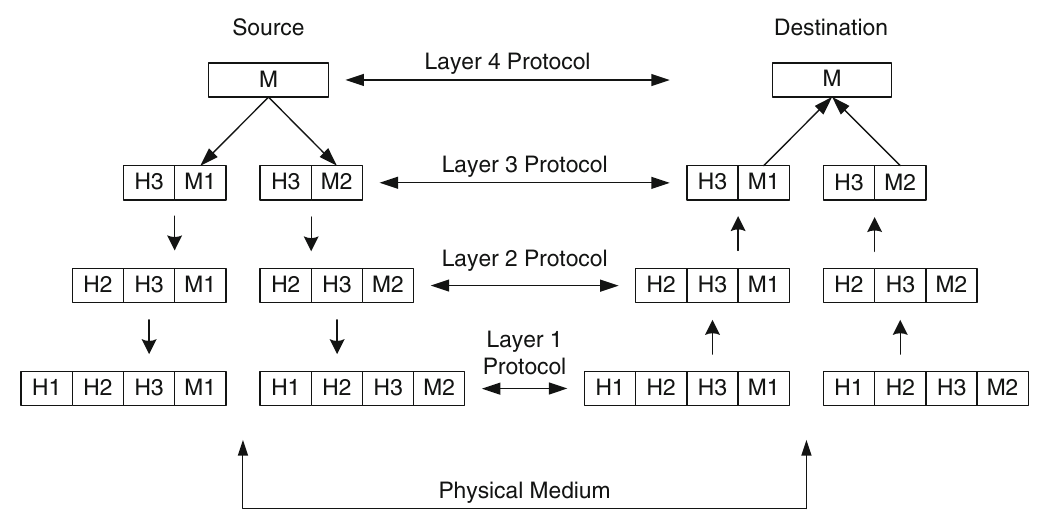
\includegraphics[width=\linewidth]{img/img001}
	\end{center}	
\end{frame}

\subsection{OSI Model}
\begin{frame}
	\frametitle{OSI Model}	
	\begin{itemize}
		\item  Open Systems Interconnection (OSI) model: reference model yang pertama kali dikembangkan oleh International Standards Organization (ISO) untuk memberikan standard framework yang menggambarkan protocol stacks di dalam computer network.
		\item Terdiri dari 7 layer dan masing-masing layer memiliki tugasnya masing-masing.
		\item Yaitu: physical layer, data link layer, network layer, transport layer, session layer, presentation layer, and application layer.
	\end{itemize}	
\end{frame}

\subsection{TCP/IP Model}
\begin{frame}
	\frametitle{TCP/IP Model}
	\begin{itemize}
		\item  TCP/IP model berdasarkan 2 protokol utama, TCP dan IP.
		\item Powerful, diimplementasikan secara luas dalam computer network saat ini.
		\item Dikembangkan oleh ARPANET, yang disponsori oleh Departemen Pertahanan Amerika Serikat.
		\item Dijuluki mbahnya computer network.
		\item Terdiri dari 5 layer: physical, data link, network, transport, dan application.
		\item Application layer $\approx$ kombinasi dari session, presentation dan application layer di OSI.
	\end{itemize}	
\end{frame}
% ----------------------------------------------------------------------------

\section{Pemodelan Sistem}
\subsection{Pendahuluan}
\begin{frame}
	\frametitle{Pemodelan Sistem}
	\begin{itemize}
		\item Pemodelan sistem: memformulasikan representasi sederhana dari sistem yang ada $\rightarrow$ agar dapat melihat sistem tanpa perlu mengimplementasikannya.
		\item Beberapa parameter dapat diberikan ke dalam model untuk mempelajari perilaku sistem.
		\item Setelah sistem telah dipelajari dengan baik $\rightarrow$ mengimplementasikan sistem.
		\item Pemodelan sistem membutuhkan asumsi-asumsi sederhana $\rightarrow$ model lebih jelas dan lebih mudah diimplementasikan.
		\item Asumsi yang berlebihan $\rightarrow$ representasi sistem tidak akurat.
		\item Ada 2 pendekatan dalam pemodelan sistem: pendekatan analitik dan pendekatan simulasi.
	\end{itemize}
\end{frame}

\subsection{Pendekatan Analitik}
\begin{frame}
	\frametitle{Pendekatan Analitik}
	\begin{itemize}
		\item Pendekatan analitik: mencari cara agar dapat menggambarkan sistem secara matematis.
		\item Menerapkan metode numerik untuk mendapatkan model matematis tsb.
		\item Biasanya menggunakan teori probabilitas dan queuing.
		\item Modelnya akan benar selama kondisi yang mendasari persamaan tersebut masih ada dan tetap.
	\end{itemize}
\end{frame}

\subsection{Pendekatan Simulasi}
\begin{frame}
	\frametitle{Pendekatan Simulasi}
	\begin{itemize}
		\item Menciptakan kembali real-world scenario menggunakan suatu program komputer.
		\item Membutuhkan lebih sedikit asumsi penyederhanaan yang sedikit, karena hampir setiap detail spesifikasi dapat dimasukkan ke dalam model simulasi.
		\item Jika sistemnya sangat besar dan kompleks, maka pendekatan analitik menjadi tidak layak.
		\item Solusinya menggunakan pendekatan simulasi.
		\item Simulasi:
		\begin{enumerate}
			\item planning,
			\item implementating (initialization, result generation, postsimulation processing),
			\item testing.
		\end{enumerate}
	\end{itemize}
\end{frame}

\begin{frame}
	\frametitle{Software Network Simulation}
	\begin{enumerate}
		\item NS2 / The Network Simulator
		\item GNS3 / Graphical Network Simulator
		\item Cisco Packet Tracer
		\item Huawei Network Tracer
	\end{enumerate}
\end{frame}

\begin{frame}
	\begin{center}
		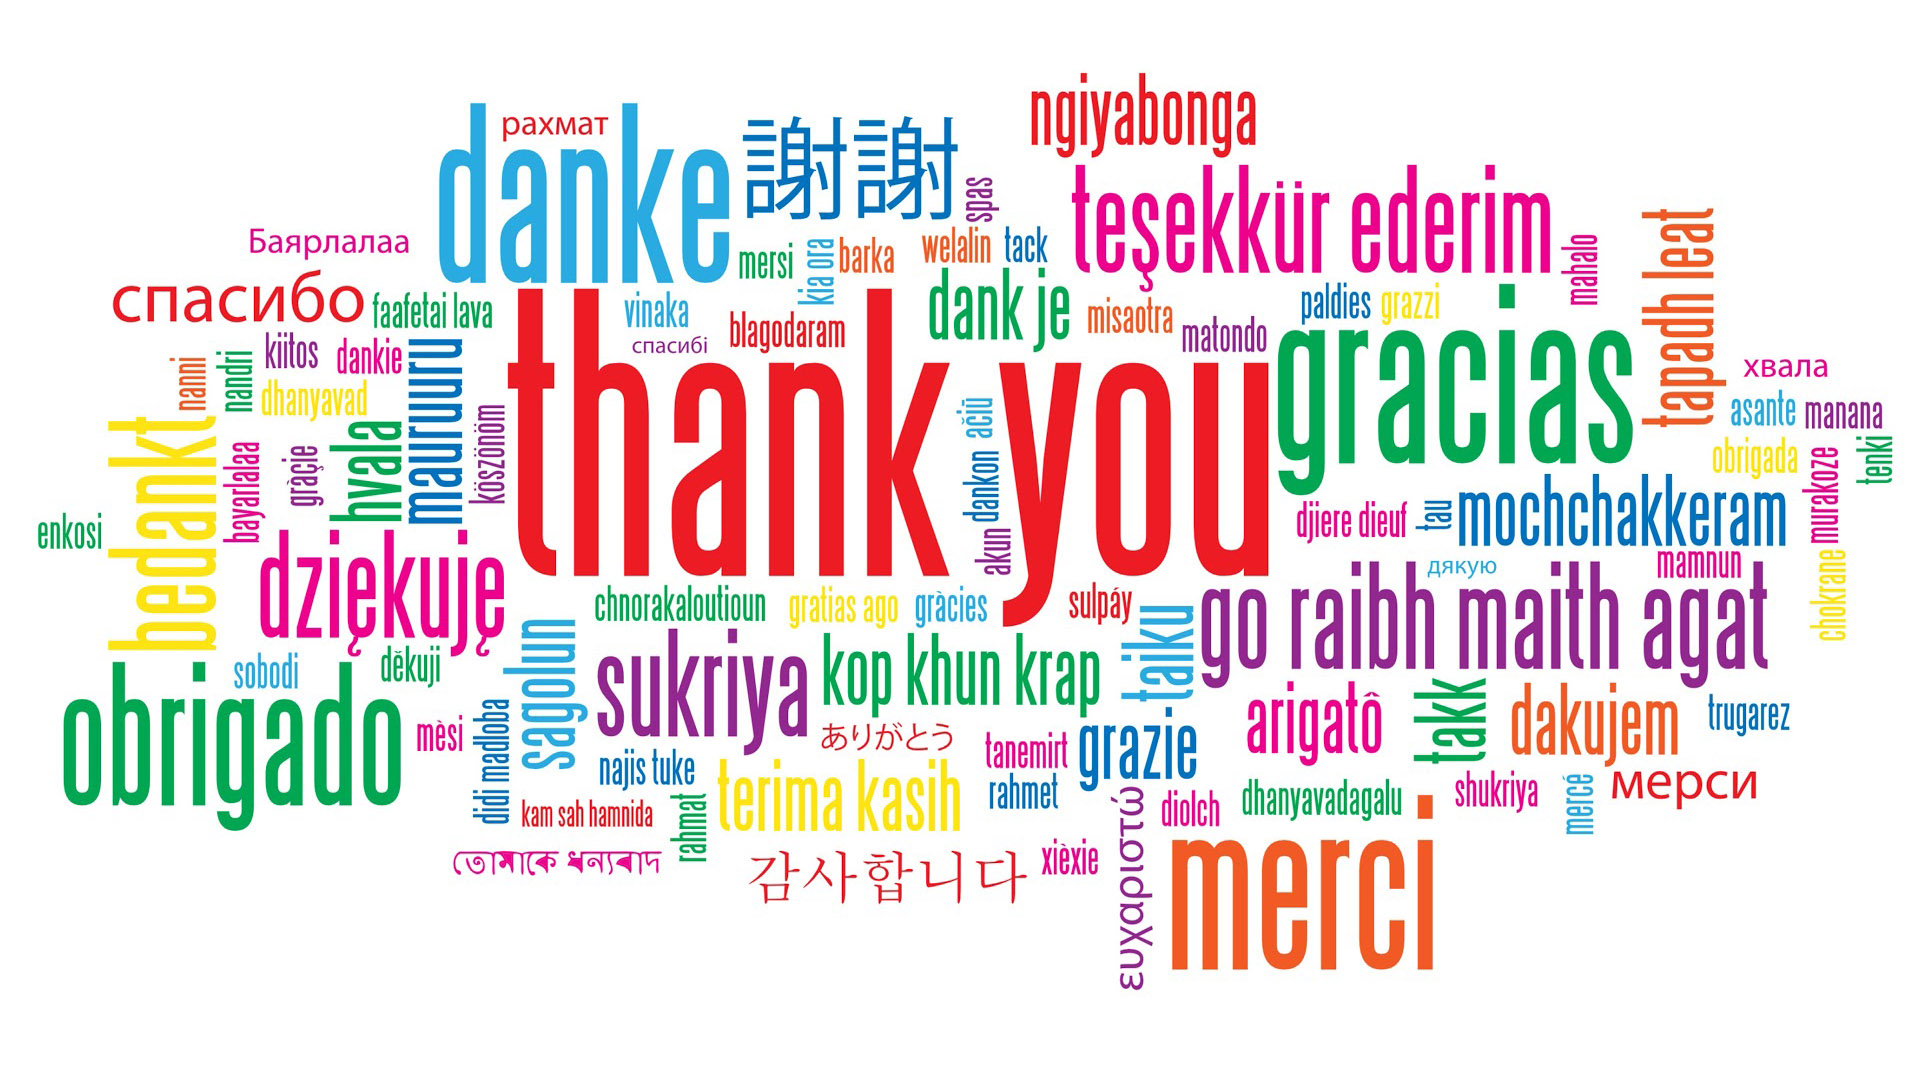
\includegraphics[width=\linewidth]{../../img/thank_you}
	\end{center}
\end{frame}


\end{document}